\section{Zusammenfassung und Diskussion}

In Versuch 256 untersuchten wir das Phänomen der Röntgenfluoreszenz. Dies ist eine sekundäre Röntgenstrahlung welche abgestrahlt wird, wenn durch einfallende Röntgen-strahlung in einem Material Elektronenübergange hervorgerufen werden. Das abgestrahlte Spektrum zeigt die aus dem vorherigen Versuch bekannten $K_{\alpha}$- und $K_{\beta}$-Linien auf, welche charakteristisch für das bestrahlte Material sind. Angenähert folgt die bei einem Elektronenübergang auf den Schalen $n_2 \to n_1$ abgestrahlte Energie dem Moseleyschen Gesetz
\begin{align}
  \sqrt{E} = \sqrt{E_R} (Z - \sigma_{n_1,n_2}) \qty(\frac{1}{n_1^2} - \frac{1}{n_2^2}).
\end{align}

Im ersten Versuchsteil bestimmten wir die Rydberg-Energie $E_R$, sowie die Abschirmkonstante $\sigma_{12}$ für Übergänge $2 \to 1$, also $K_{\alpha}$-Übergänge, und  $\sigma_{13}$ für Übergänge $3 \to 1$, also $K_{\beta}$-Übergänge. Hierzu nahmen wir zunächst die Röntgenfluoreszenzspektren verschiedener reiner Metalle auf. Durch die Analysesoftware wurden die gemessenen abgestrahlten Energieimpulse entsprechend ihrer Stärke in Kanälen kategorisiert. Um damit rechnen zu können, mussten wir die Energieskala kalibrieren, indem wir die bekannten Energien der $K_{\alpha}$-Übergänge von Eisen und Molybdän mit den entsprechenden Kanälen, in welchen wir die Peaks fanden assoziieren. In \tabref{tab:elemente_kalph_kbeta_vergleich} sind die ermittelten Energiewerte der Linien zusammen mit den Literaturwerten\footnote{Quelle Literaturwerte Energien: https://physics.nist.gov/PhysRefData/XrayTrans/Html/search.html} zum Vergleich zu finden.


\begin{table}[H]
  \centering
  \begin{tabular}{|c|c|c|c|c|c|c|c|}
      \hline
      \# & Element & $E_{\alpha}\ [\si{\kilo\electronvolt}]$ & $E_{\alpha,\text{Lit}}\ [\si{\kilo\electronvolt}]$ & Abw. & $E_{\beta}\ [\si{\kilo\electronvolt}]$ & $E_{\beta,\text{Lit}}\ [\si{\kilo\electronvolt}]$ & Abw.  \\
      \hline
      1  & Mo  & $17.46 \pm 0.18$ & $-$ & $-$ & $19.57 \pm 0.17$ & $19.61$ & $0.24\sigma$\\
      2  & Fe     & $6.38  \pm 0.17$ & $-$ & $-$ & $7.03  \pm 0.42$ & $7.06$ & $0.08\sigma$\\
      3  & Ni    & $7.46  \pm 0.18$ & $7.48$ & $0.12\sigma$ & $8.26  \pm 0.21$ & $8.27$ & $0.05\sigma$\\
      4  & Zn      & $8.64  \pm 0.18$ & $8.64$ & $0$ & $9.59  \pm 0.16$ & $9.57$ & $0.13\sigma$\\
      5  & Zr & $15.78 \pm 0.18$ & $15.77$ & $0.06\sigma$ & $17.67 \pm 0.19$ & $17.67$ & $0$\\
      6  & Ti     & $4.44  \pm 0.19$ & $4.51$ & $0.37\sigma$ & $4.44  \pm 0.19$ & $4.93$ & $2.58\sigma$\\
      7  & Cu    & $8.04  \pm 0.17$ & $8.05$ & $0.06\sigma$ & $8.91  \pm 0.14$ & $8.91$ & $0$\\
      8  & Ag    & $21.89 \pm 0.21$ & $22.16$ & $1.29\sigma$ & $24.59 \pm 0.18$ & $24.94$ & $1.95\sigma$\\
      \hline
  \end{tabular}
  \caption{Energien der $K_{\alpha}$- und $K_{\beta}$-Linien der untersuchten Elemente und Vergleich mit den entsprechenden Literaturwerten.}
  \label{tab:elemente_kalph_kbeta_vergleich}
\end{table}

Nacheinander trugen wir einem die $K_{\alpha}$-Energien und einmal die $K_{\beta}$-Energien über der Kernladungszahl $Z$ der Elemente in einem Diagramm auf und passten die oben genannte Funktion an diese Daten an.
Aus der Anpassung an die $K_{\alpha}$-Energie ermittelten wir so die Werte
\begin{align}
  \sigma_{12} &= 1.4 \pm 0.5
\intertext{und}
  E_R &= (14.1 \pm 0.4) \si{\electronvolt}.
\end{align}

Im Vergleich mit dem Wert von etwa $13.6\si{\electronvolt}$ aus der Praktikumsanleitung weicht der von uns berechnete Wert um etwa $1.54\sigma$ ab. Der ermittelte Wert von $\sigma_{12}$ weicht um etwa $1.03\sigma$ vom Literaturwert\footnote{Quelle Literaturwerte $\sigma_{12}$, $\sigma_{13}$: https://de.wikipedia.org/wiki/Moseleysches\_Gesetz} von ungefähr $1.0$ ab.

Aus der Anpassung der Funktion an die $K_{\beta}$-Energien konnten wir die Werte
\begin{align}
  \sigma_{13} &= 2.2 \pm 0.4
\intertext{und}
  E_R &= (13.87 \pm 0.21) \si{\electronvolt}.
\end{align}
bestimmen.

Der hier für $E_R$ berechnete Wert weicht ebenfalls um etwa $1.54\sigma$ vom Literaturwert ab. Die Abweichung des von uns ermittelten Wertes von $\sigma_{13}$ zum Literaturwert von etwa $1.8$ beträgt ungefähr $1.13\sigma$.

Die bekannten Positionen der $K_{\alpha}$- und $K_{\beta}$-Linien im Röntgenfluoreszenzspektrum eines Metalls lassen sich außerdem verwenden, um die Bestandteile von Metalllegierungen herauszufinden. Um dies zu erproben, untersuchten wir im abschließenden Versuchsteil die Röntgenfluoreszenzspektren fünf verschiedener Metalllegierungen. Hierunter fanden wir die folgenden Legierungen:
\begin{itemize}
  \item Eisen + Chrom = Ferrochrom(?)
  \item Kupfer + Zink = Messing (zwei Mal)
  \item Eisen + Nickel = Invar(?)
  \item Kupfer + Gallium + Germanium = ?
\end{itemize}

Die aufgezeichneten Spektren sind noch einmal in den Abbildungen \abbref{fig:legierung1_zsmf} und \abbref{fig:legierung2345_zsmf} zusammengefasst zu sehen.


\begin{figure}[H]
  \centering
  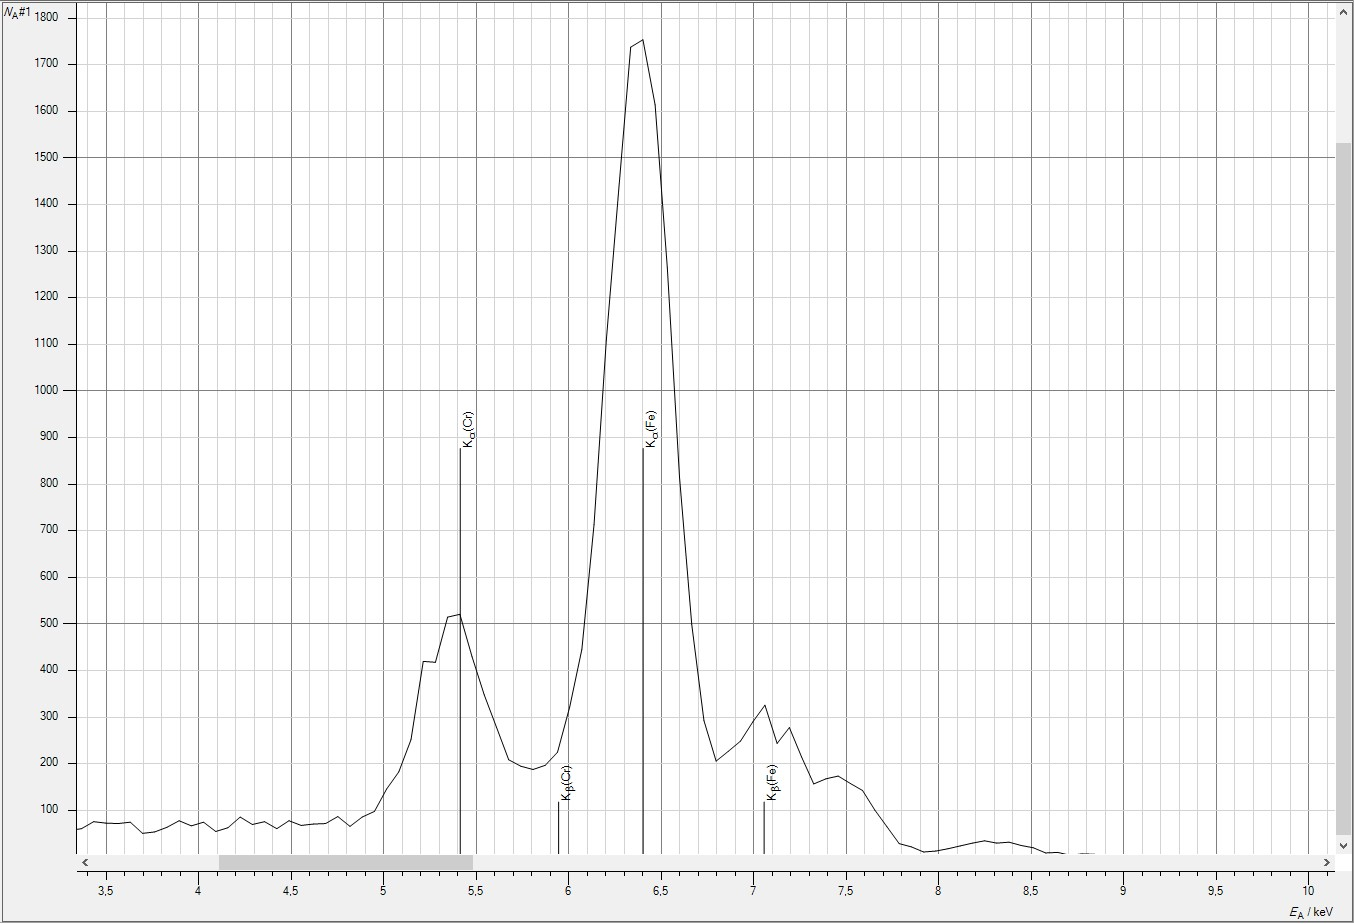
\includegraphics[width=\textwidth]{files/legierung1.jpg}
  \caption{Legierung 1: Eisen + Chrom}
  \label{fig:legierung1_zsmf}
\end{figure}

\begin{figure}[H]
  \centering
  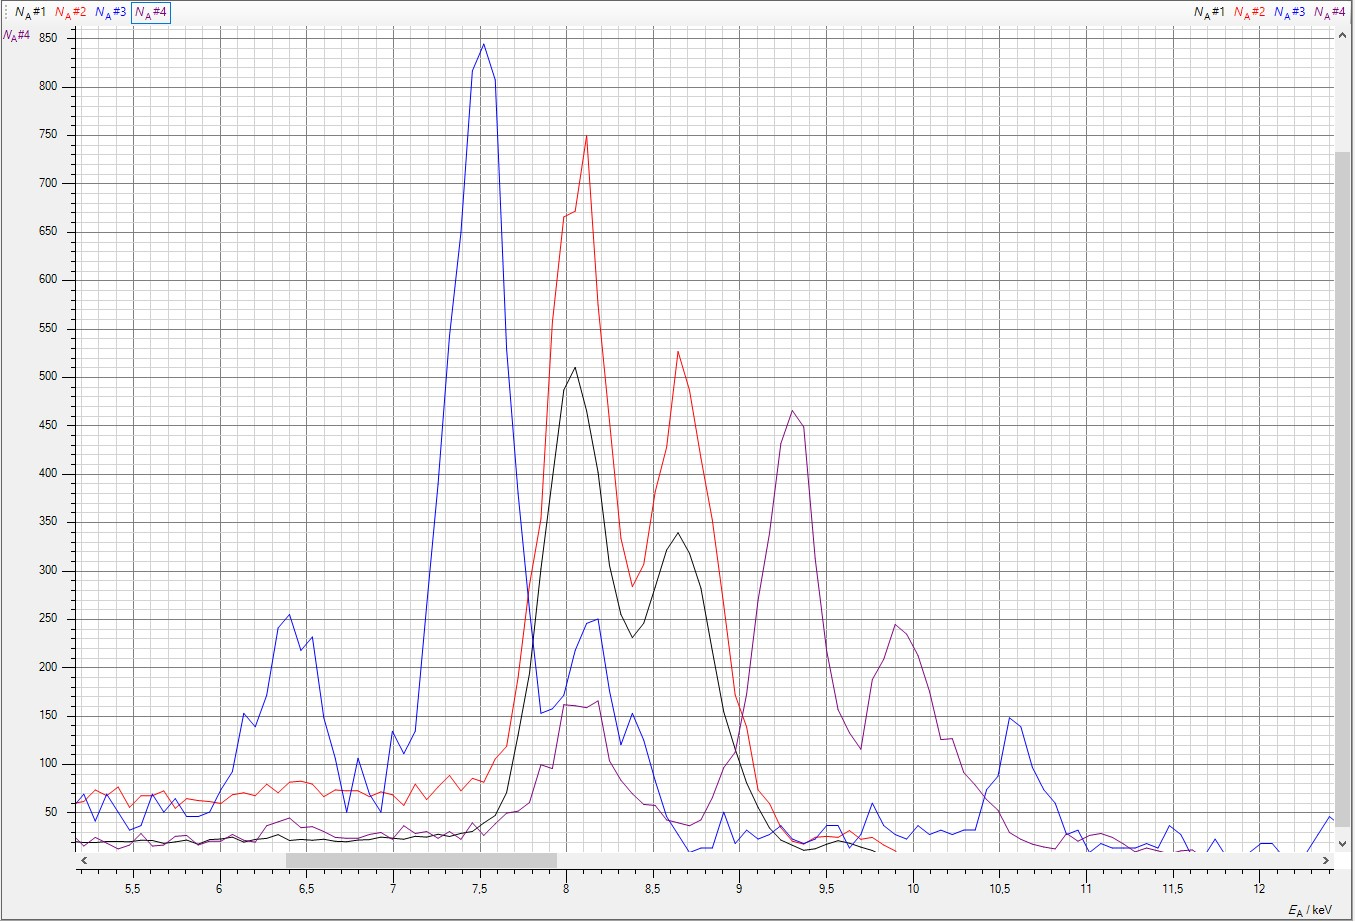
\includegraphics[width=\textwidth]{files/legierung2345.jpg}
  \caption{Legierungen 2 - 5}
  \label{fig:legierung2345_zsmf}
\end{figure}